\documentclass[conference]{IEEEtran}
\usepackage{amsmath,amssymb}
\usepackage{booktabs}
\usepackage{graphicx}
\usepackage{subcaption}
\usepackage{hyperref}

% Makes the figure paths below resolve whether pdflatex is run from the repo
% root (fixed-k5/, where `assets/...` is the correct relative path) or from
% inside docs/ (where the real path is `../assets/...`). Tries both parent
% directories so the existing `assets/...` filenames in \includegraphics
% below don't need to change.
\graphicspath{{../}{./}}

% Float placement tuning: figure* (double-column) floats in IEEEtran's
% two-column layout are otherwise prone to being pushed to the very end of
% a short paper. Combined with moving the figure*'s source position (see
% below), this keeps Fig. 1 near page 2 instead of the last page.
\renewcommand{\topfraction}{0.9}
\renewcommand{\bottomfraction}{0.9}
\renewcommand{\textfraction}{0.07}
\renewcommand{\floatpagefraction}{0.7}
\renewcommand{\dbltopfraction}{0.9}
\renewcommand{\dblfloatpagefraction}{0.7}

\begin{document}

\title{Fixed-K Speculative Decoding for Energy-Proportional LLM Serving: \\
A Reproducible Empirical Validation}

\author{
\IEEEauthorblockN{Zanno Jacklin}
\IEEEauthorblockA{Independent Researcher, Creepybits}
}

\maketitle

\begin{figure*}[!t]
\centering
\begin{subfigure}{0.48\textwidth}
\centering
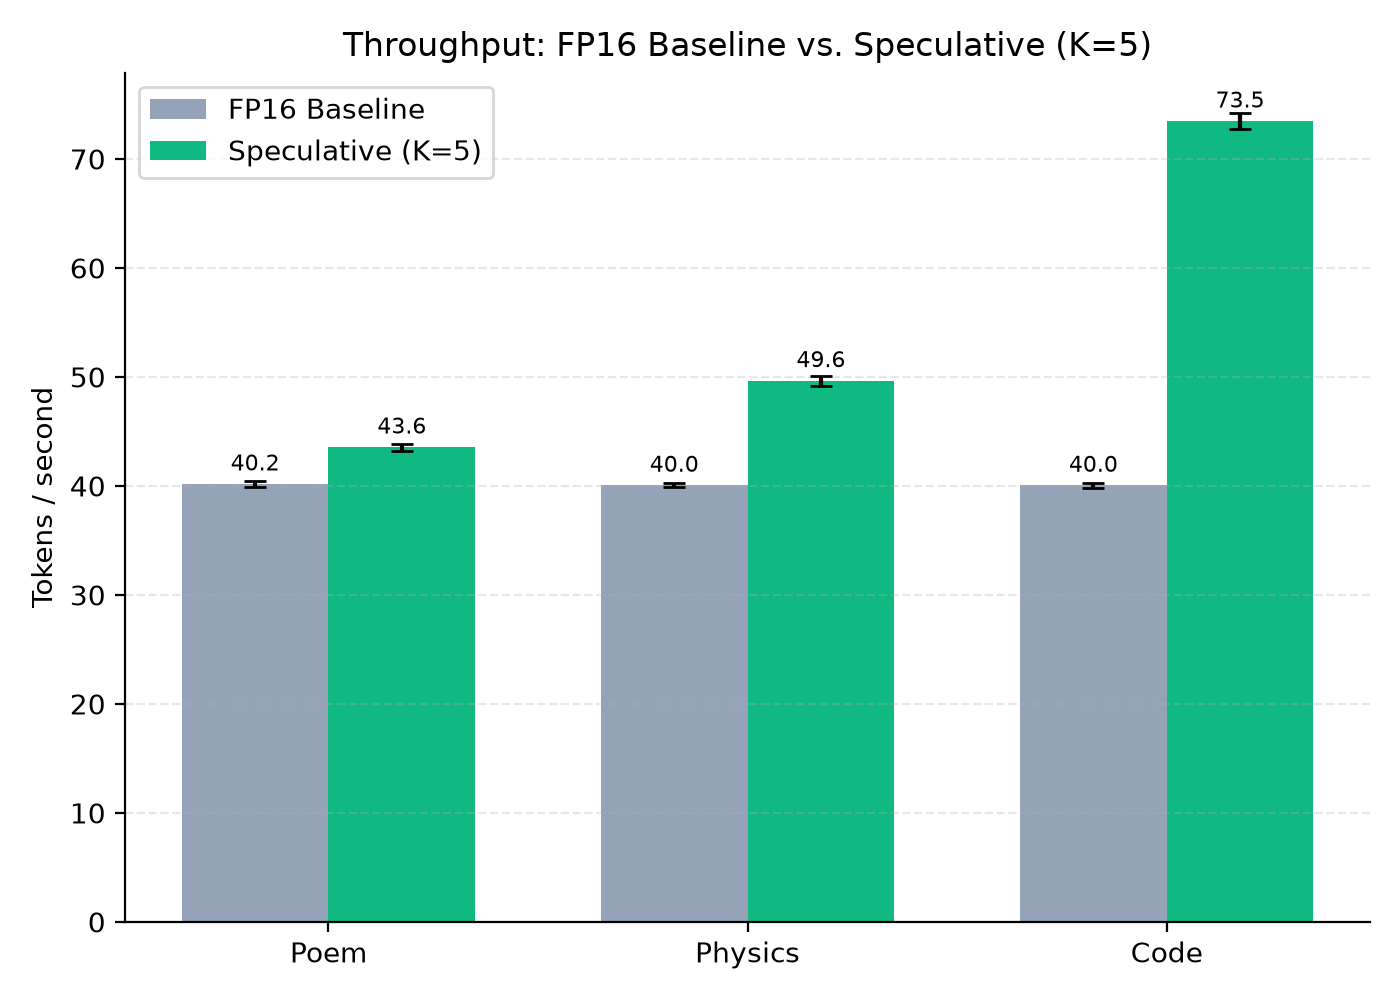
\includegraphics[width=\linewidth]{assets/throughput_baseline_vs_speculative.png}
\caption{Throughput}
\label{fig:throughput}
\end{subfigure}
\hfill
\begin{subfigure}{0.48\textwidth}
\centering
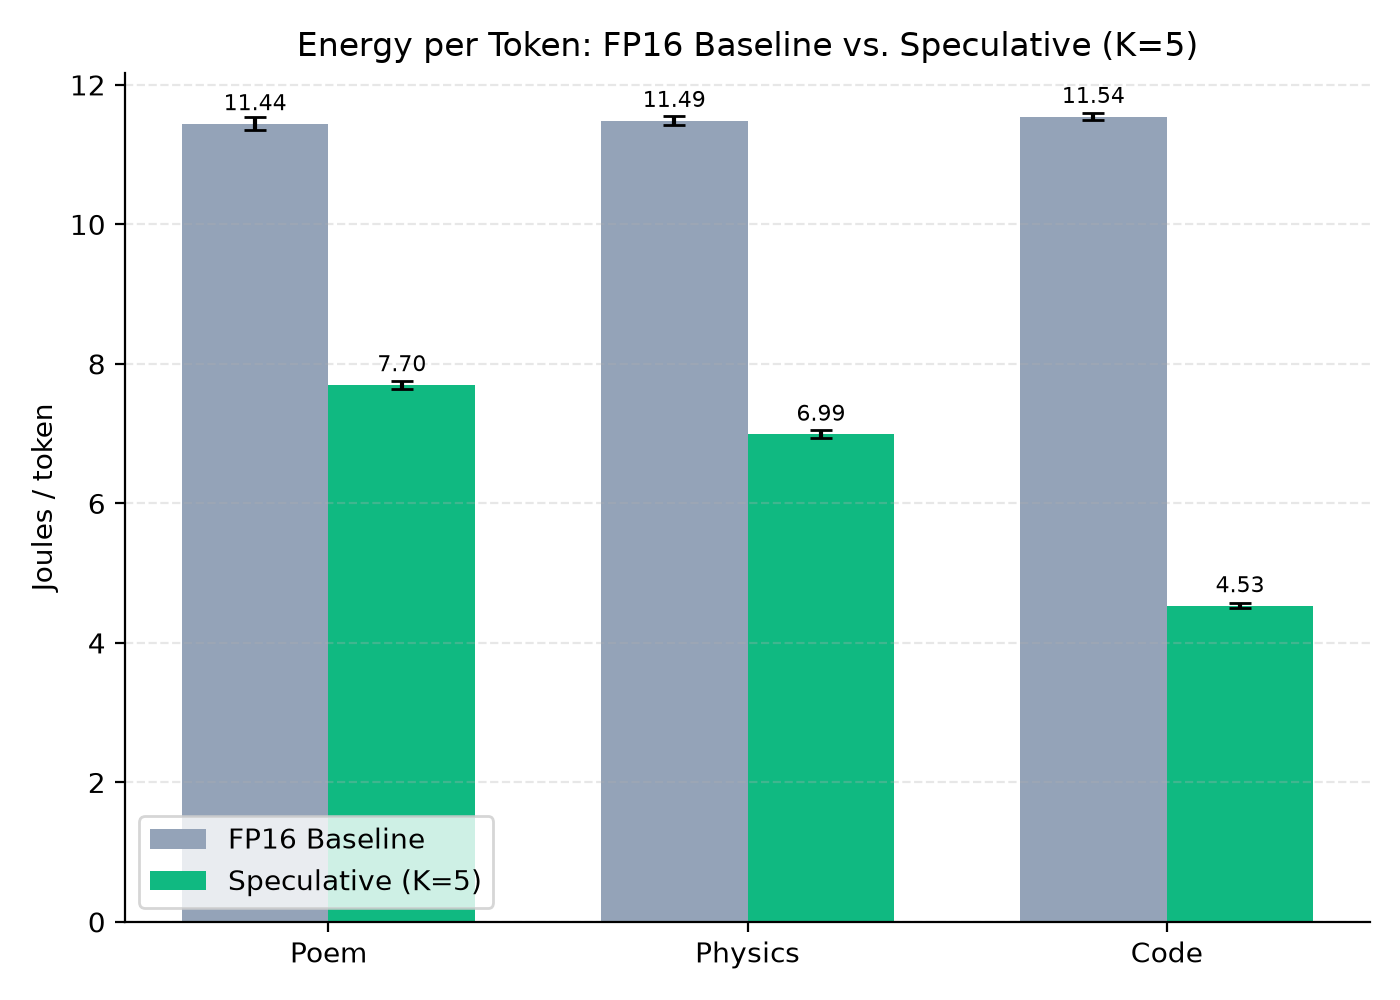
\includegraphics[width=\linewidth]{assets/energy_per_token_baseline_vs_speculative.png}
\caption{Energy per token}
\label{fig:energy}
\end{subfigure}
\caption{FP16 baseline vs. fixed-$K{=}5$ speculative decoding, per prompt (N=10 trials/prompt, error bars show $\pm 1$ std. dev.). Gains are smallest on the least predictable content (Poem) and largest on the most predictable (Code).}
\label{fig:throughput_energy}
\end{figure*}

\begin{abstract}
We present an empirical validation of fixed draft-length ($K{=}5$) speculative
decoding using a scout(1B)$\to$target(8B) model pair on consumer GPU hardware.
Across three prompt categories spanning low to high output determinism (creative
poetry, technical explanation, and code generation), we measure throughput,
energy per token, and output fidelity relative to a matched FP16 autoregressive
baseline. Speculative decoding achieves up to +83.5\% throughput
improvement and $-$60.8\% energy reduction per token on
code generation, with smaller but consistent gains on less predictable prose
(+8.4\% / $-$32.7\% on poetry). All results
achieve 100\% exact-token-match fidelity against the baseline (lossless,
greedy decoding) and are independently reproducible from the accompanying
open-source repository. We report results transparently, including the
deliberate methodological choice to omit KV-caching from both arms of the
comparison, which keeps the relative comparison fair but means absolute
throughput figures are not representative of a production-optimized server,
and including two documented measurement-methodology corrections (a
warmup-timing bug, and subsequently a warmup convergence-criterion bug, both
affecting earlier versions of this result) alongside the closed-loop warmup
convergence and residual-drift diagnostics that caught them and now guard
against a recurrence.
\end{abstract}

\begin{IEEEkeywords}
speculative decoding, energy-efficient inference, large language models, GPU power measurement
\end{IEEEkeywords}

\section{Introduction}

Autoregressive decoding in large language models (LLMs) is inherently
sequential: each output token requires a full forward pass through the
target model before the next token can be produced. This serial dependency
underutilizes modern GPU compute, which is optimized for parallel throughput.
Speculative decoding~\cite{leviathan2023fast,chen2023accelerating} addresses
this by using a smaller, faster \emph{scout} model to propose a short window
of candidate tokens, which the larger \emph{target} model then verifies in a
single parallel forward pass, accepting the longest correct prefix.

This paper reports a narrow, fully-validated empirical claim: a fixed draft
window of $K{=}5$ tokens, paired with an exact (lossless) accept/reject
verification scheme, produces measurable throughput and energy improvements
on real consumer GPU hardware, with perfect output fidelity relative to
standard greedy decoding. We deliberately scope this paper to only the
mechanism we have fully validated. A related, more ambitious mechanism
under investigation in the parent project --- entropy-gated \emph{dynamic}
adjustment of the draft window, intended to switch between aggressive and
conservative speculation based on local output entropy --- is explicitly
\textbf{not} included here, as it has not yet been shown to outperform this
simpler fixed-$K$ approach in single-request testing.

\subsection{Relationship to prior work}

Entropy-gated adaptive speculative decoding is an active research area.
AdaEDL~\cite{adaedl2024} reports 10--57\% improvement over static draft
length using entropy-based adaptive drafting. SGLang ships a built-in
adaptive speculative-length mechanism using an EMA of accepted draft length.
Our own testing of an entropy-gated variant, using the same hardware and
methodology as this paper, has not yet demonstrated an improvement over the
simpler fixed-$K$ approach reported here; we regard that as an open question
requiring further work (e.g. testing under multi-request/batched serving,
which published entropy-gating results suggest is where the technique's
value proposition may actually lie), not a settled negative result. This
paper makes no claims about the entropy-gated mechanism in either direction.

\section{Methodology}

\subsection{Models and hardware}

Scout model: Llama-3.2-1B-Instruct. Target model: Llama-3.1-8B-Instruct.
Both loaded in bfloat16. All measurements taken on a single NVIDIA RTX 5090
(Blackwell architecture) GPU, single-request (batch size 1), greedy
(argmax) decoding throughout. The results reported here were collected under
WSL2, without NVML GPU clock locking (no elevated privileges available in
that environment); this is noted for reproducibility, since clock-locked runs
would be expected to show lower run-to-run variance.

\subsection{Draft-verify procedure}

At each decoding cycle, the scout model autoregressively proposes $K{=}5$
candidate tokens. The target model then performs a single forward pass over
the full draft sequence, and its argmax predictions at each position are
compared against the corresponding drafted tokens. The longest matching
prefix is accepted; at the first mismatch (or after all $K$ tokens match),
the target's own prediction is substituted, exactly reproducing what
standard greedy decoding would have produced at that position. This
verification scheme is lossless by construction: the output token sequence
is provably identical, position-for-position, to what running the target
model alone would produce, since every emitted token is either a drafted
token confirmed by the target's own argmax, or the target's argmax directly.

\subsection{Power and energy measurement}

GPU power is sampled via NVML at 100~Hz on a background thread throughout
each timed generation window. Energy per token is read from the GPU's
onboard hardware energy counter
(\texttt{nvmlDeviceGetTotalEnergyConsumption}) when available, as it was for
every trial reported in this paper, divided by $N_{\text{tok}}$, the number
of tokens produced. This is a more direct measurement than integrating
sampled instantaneous power readings, which is retained in the accompanying
code only as a fallback and cross-check for hardware that lacks the counter.

\subsection{Warmup}
\label{sec:warmup-correction}

Warmup is applied in two layers. First, a one-time \emph{closed-loop thermal
warmup} runs real, discarded decoding cycles -- alternating across all
prompts and both the baseline and speculative conditions -- until, for each
individual prompt/condition combination separately, both its power reading
and its die-temperature reading stop drifting relative to their own recent
history. Checking per-combination rather than pooled matters for two
independent reasons found in sequence. One: baseline and speculative
decoding draw genuinely different power by design; a convergence check that
simply requires consecutive readings to agree with each other, without
accounting for which workload produced them, can fail to terminate when the
workload alternates between conditions with a real, persistent power gap.
The other, found only after fixing the first issue: die temperature is not
actually workload-independent on this hardware -- baseline and speculative
decoding settle at temperatures roughly 3--4$^\circ$C apart, so pooling
temperature across both (on the assumption that it is a slow,
workload-independent signal) produces a permanent oscillation in the
rolling window that no absolute tolerance can ever satisfy, regardless of
run length. A separate, independent issue affected the power check alone:
an absolute tolerance of 1.5~W was tighter than the hardware's own
sample-to-sample noise floor (measured standard deviation 2.9~W at
baseline load, 6.8~W at speculative load), making it unsatisfiable on its
own terms. All three are corrected in the procedure used for this paper:
warmup burst length matches the real trial length (an earlier version used
a shorter burst, which was found empirically to converge at a lower
power/thermal level than the real, longer trial then reached); power and
temperature are both tracked per prompt/condition combination rather than
pooled; and convergence for both is judged by a half-split drift statistic
(the difference between the mean of the newer half and the older half of a
rolling window) against a tolerance relative to each combination's own mean
(1.5\% for power, 1$^\circ$C absolute for temperature, empirically already
well above its own noise floor), rather than raw min-max spread, which
grows with window length under pure noise and does not isolate drift from
noise the way a half-split comparison does. Second, independently of the
closed-loop warmup above, each individual timed trial is still preceded by 5
short untimed forward-pass warmup steps immediately before its own
measurement window, avoiding cold-SM effects specific to that trial. This
two-layer procedure is shared between both arms of the comparison
(\texttt{benchmark\_ablation.py} and \texttt{speculative\_scout.py}) via a
common \texttt{bench\_common.py} module.

\subsection{Deliberate exclusion of KV-caching}

Both the baseline and speculative decoding paths recompute attention over
the full sequence at every step, with no KV-cache reuse. This was a
deliberate methodological choice: an earlier iteration of this work applied
caching only to the baseline arm, which structurally penalized the
speculative path whenever it fell back to single-step generation (a full
uncached recompute for a single token is the worst-case cost ratio in the
system). Removing caching from both arms restores a fair relative
comparison at the cost of both arms being substantially slower in absolute
terms than a production server with caching would be. We therefore report
\emph{relative} throughput and energy figures as the validated result, and
explicitly flag that absolute tok/s numbers in this paper are not
production-representative.

\subsection{Fidelity measurement}

Fidelity is measured as the exact token-for-token match rate between the
baseline's greedy output and the speculative path's output, over the full
generated sequence, for each prompt.

\subsection{Prompts}

Three prompts were selected to span a range of output determinism:
\begin{itemize}
\item \textbf{Poem} (low determinism): an open-ended creative writing task
(an original Chant Royal poem on a mathematical theme).
\item \textbf{Physics} (medium determinism): a technical explanation task
(semiconductor memory bandwidth and the memory wall).
\item \textbf{Code} (high determinism): a code-generation task (a Python
binary search tree implementation with type annotations), where correct
completions are far more constrained token-to-token.
\end{itemize}

\section{Results}
\label{sec:results}

\subsection{Fidelity}

Aggregate exact-token-match fidelity across all three prompts was
100.0\%, confirming the accept/reject implementation is lossless
in practice as well as by construction.

\subsection{Throughput, energy, and power}

Table~\ref{tab:results} reports mean $\pm$ standard deviation across
$N{=}10$ trials per prompt per condition.

\begin{table*}[t]
\centering
\caption{Baseline vs. fixed-$K{=}5$ speculative decoding, per prompt. N=10 trials/prompt. Collected 2026-09-05, the first run with a fully converged closed-loop warmup (see Section~\ref{sec:validity}).}
\label{tab:results}
\begin{tabular}{lccccccc}
\toprule
Prompt & Baseline tok/s & Spec. tok/s & Speedup & Baseline J/tok & Spec. J/tok & Energy $\Delta$ & Accept \% \\
\midrule
Poem     & 40.16 $\pm$ 0.28 & 43.55 $\pm$ 0.31 & +8.4\% & 11.44 $\pm$ 0.09 & 7.70 $\pm$ 0.06 & $-$32.7\% & 42.5\% \\
Physics  & 40.05 $\pm$ 0.18 & 49.64 $\pm$ 0.43 & +24.0\% & 11.49 $\pm$ 0.06 & 6.99 $\pm$ 0.06 & $-$39.2\% & 51.7\% \\
Code     & 40.04 $\pm$ 0.23 & \textbf{73.46 $\pm$ 0.74} & \textbf{+83.5\%} & 11.54 $\pm$ 0.05 & \textbf{4.53 $\pm$ 0.04} & \textbf{$-$60.8\%} & \textbf{85.4\%} \\
\bottomrule
\end{tabular}
\end{table*}

Mean GPU power during speculative decoding (346--364~W) is
lower than during FP16 baseline decoding
(463--466~W), despite two models being resident in VRAM
simultaneously. This is consistent with fewer full 8B-parameter forward
passes being required per unit of output as accepted draft batch length
grows -- each accepted cycle of up to $K{+}1{=}6$ tokens requires only one
target forward pass, versus six for the baseline. Accept rates (42.5\% /
51.7\% / 85.4\%) and per-prompt throughput/energy figures both agree
closely with an independent single-run measurement from
\texttt{speculative\_scout.py} (a separate script sharing only
\texttt{bench\_common.py}, not the trial-averaging logic), which we take as
further evidence against measurement artifacts specific to either script.

\subsection{Measurement validity: residual drift diagnostics}
\label{sec:validity}

After the corrections to the warmup procedure described in
Section~\ref{sec:warmup-correction}, each run's per-trial telemetry is
checked for residual drift: a least-squares fit of power, energy/token, and
throughput against chronological trial index within the run. The run behind
Table~\ref{tab:results} is the first on this project with a closed-loop
warmup that fully converged within its time cap (241.3~s, well under the
420~s cap; every prior run had hit the cap without converging) and the
cleanest drift diagnostics observed to date: the fitted trend was
negligible for every metric, pooled and per-condition ($R^2$ between
$4\times10^{-5}$ and $0.037$ across all cases), and the accompanying code's
pass/fail threshold ($\pm 0.5\%$ of the mean) passed cleanly on every check
(pooled $0.30\%$; baseline-only $0.38\%$; speculative-only $0.19\%$) --
unlike earlier runs, where the threshold fired despite a near-zero $R^2$ and
had to be interpreted rather than simply read off. We treat the results in
Table~\ref{tab:results} as the most reliable of this project to date on that
basis.

\subsection{Speedup and energy reduction scale with acceptance rate}

Figure~\ref{fig:speedup_accept} shows speedup tracking draft acceptance
rate across the three prompts, consistent with the mechanism's expected
behavior: more predictable continuations (code) allow the scout to
correctly anticipate more tokens per cycle, directly translating to fewer
expensive target forward passes.

\begin{figure}[t]
\centering
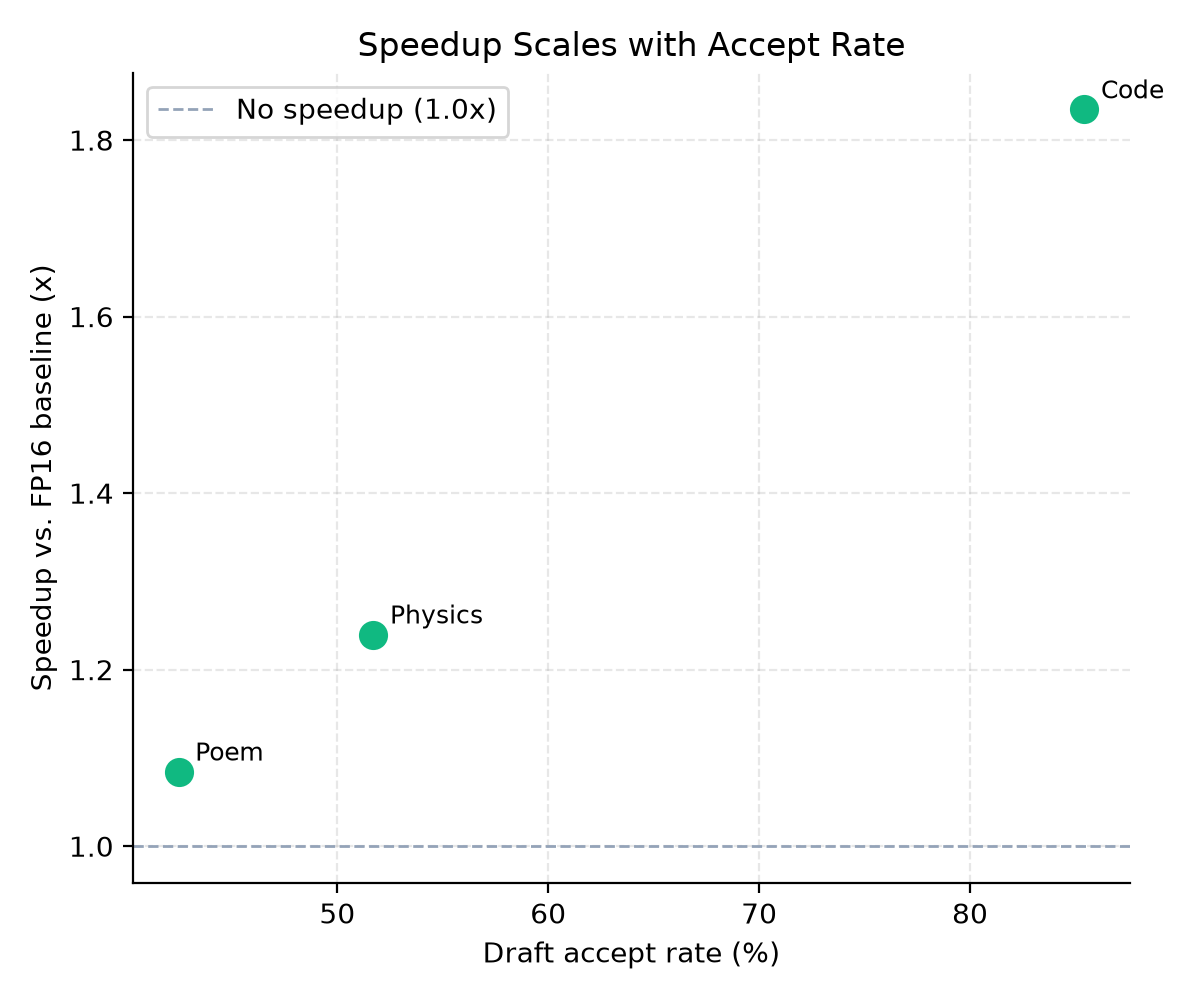
\includegraphics[width=0.9\linewidth]{assets/speedup_vs_accept_rate.png}
\caption{Speedup vs. FP16 baseline as a function of draft accept rate, across the three prompts. The relationship is monotonic and consistent with the mechanism's expected behavior.}
\label{fig:speedup_accept}
\end{figure}

\section{Discussion and Limitations}

\subsection{Absolute throughput is not production-representative}

As noted in Methodology, neither arm of this comparison uses KV-caching.
A production serving stack with proper cache reuse would show substantially
higher absolute throughput in both arms; we have not yet validated
fixed-$K$ speculative decoding's behavior under a cached, production-style
serving loop, and consider this the primary remaining gap before these
results can inform a deployment decision.

\subsection{Single-request, single-GPU scope}

All results in this paper are single-request (batch size 1) measurements
on a single consumer GPU. Behavior under batched, multi-request serving --
where the entropy-gated dynamic variant may plausibly outperform this
fixed-$K$ approach, per precedent in AdaEDL and SGLang -- is untested and
out of scope for this paper.

\subsection{Reproducibility}

All code, raw telemetry (JSON/CSV), and the scripts used to generate every
figure and table in this paper are available at
\url{https://github.com/Creepybits/sdsie-fixed-k5-speculative-decoding}
under an Apache-2.0 license. Reported numbers are directly traceable to
\texttt{telemetry/ablation\_results.json}, generated by
\texttt{benchmark\_ablation.py} in that repository. The closed-loop warmup
and drift-diagnostic logic described in Sections~\ref{sec:warmup-correction}
and~\ref{sec:validity} is shared between \texttt{benchmark\_ablation.py} and
\texttt{speculative\_scout.py} via \texttt{bench\_common.py}.

\section{Conclusion}

Fixed-$K{=}5$ speculative decoding, with an exact lossless verification
scheme, produces measurable and reproducible throughput and energy gains
on real consumer GPU hardware, scaling with output predictability, with
zero loss of output fidelity. We report this as a validated, narrow result,
distinct from and not dependent on the more experimental entropy-gated
dynamic mechanism under investigation elsewhere in the parent project.

\bibliographystyle{IEEEtran}
\begin{thebibliography}{9}

\bibitem{leviathan2023fast}
Y. Leviathan, M. Kalman, and Y. Matias,
``Fast Inference from Transformers via Speculative Decoding,''
\emph{Proc. 40th Int. Conf. Machine Learning (ICML)}, 2023.

\bibitem{chen2023accelerating}
C. Chen, S. Borgeaud, G. Irving, J.-B. Lespiau, L. Sifre, and J. Jumper,
``Accelerating Large Language Model Decoding with Speculative Sampling,''
arXiv:2302.01318, 2023.

\bibitem{adaedl2024}
Qualcomm AI Research,
``AdaEDL: Adaptive Entropy-based Dynamic Layer for Efficient Speculative Decoding,''
arXiv:2410.18351, 2024.

\end{thebibliography}

\end{document}
